\subsection{Experimental Procedure}\label{subsec:experimental-procedure}

The object of the current investigation is the operation of the experimental semi-continuous rolling plant located at the Institute of Metal Forming, TU Bergakademie Freiberg.
It consists of a two-high reversing roughing stand and four continuous finishing stands.
The pass schedule of the current work consists of 10 oval-round reversing passes followed by 4 oval-round continuous finishing passes.
A \qty{50}{\milli\meter} round workpiece made of C45 carbon steel is rolled down to \qty{8}{\milli\meter} diameter, starting at \qty{1150}{\celsius}, resp.\ \qty{1423.15}{\kelvin}.
Details of the schedule are provided in \autoref{tab:process_conditions} and in the supplemental material~\cite{WeinerVariationSupplemental2023}.
The profile shapes appearing in the schedule are illustrated in \autoref{fig:plot_pass_sequence}.

\begin{figure}
    \centering
    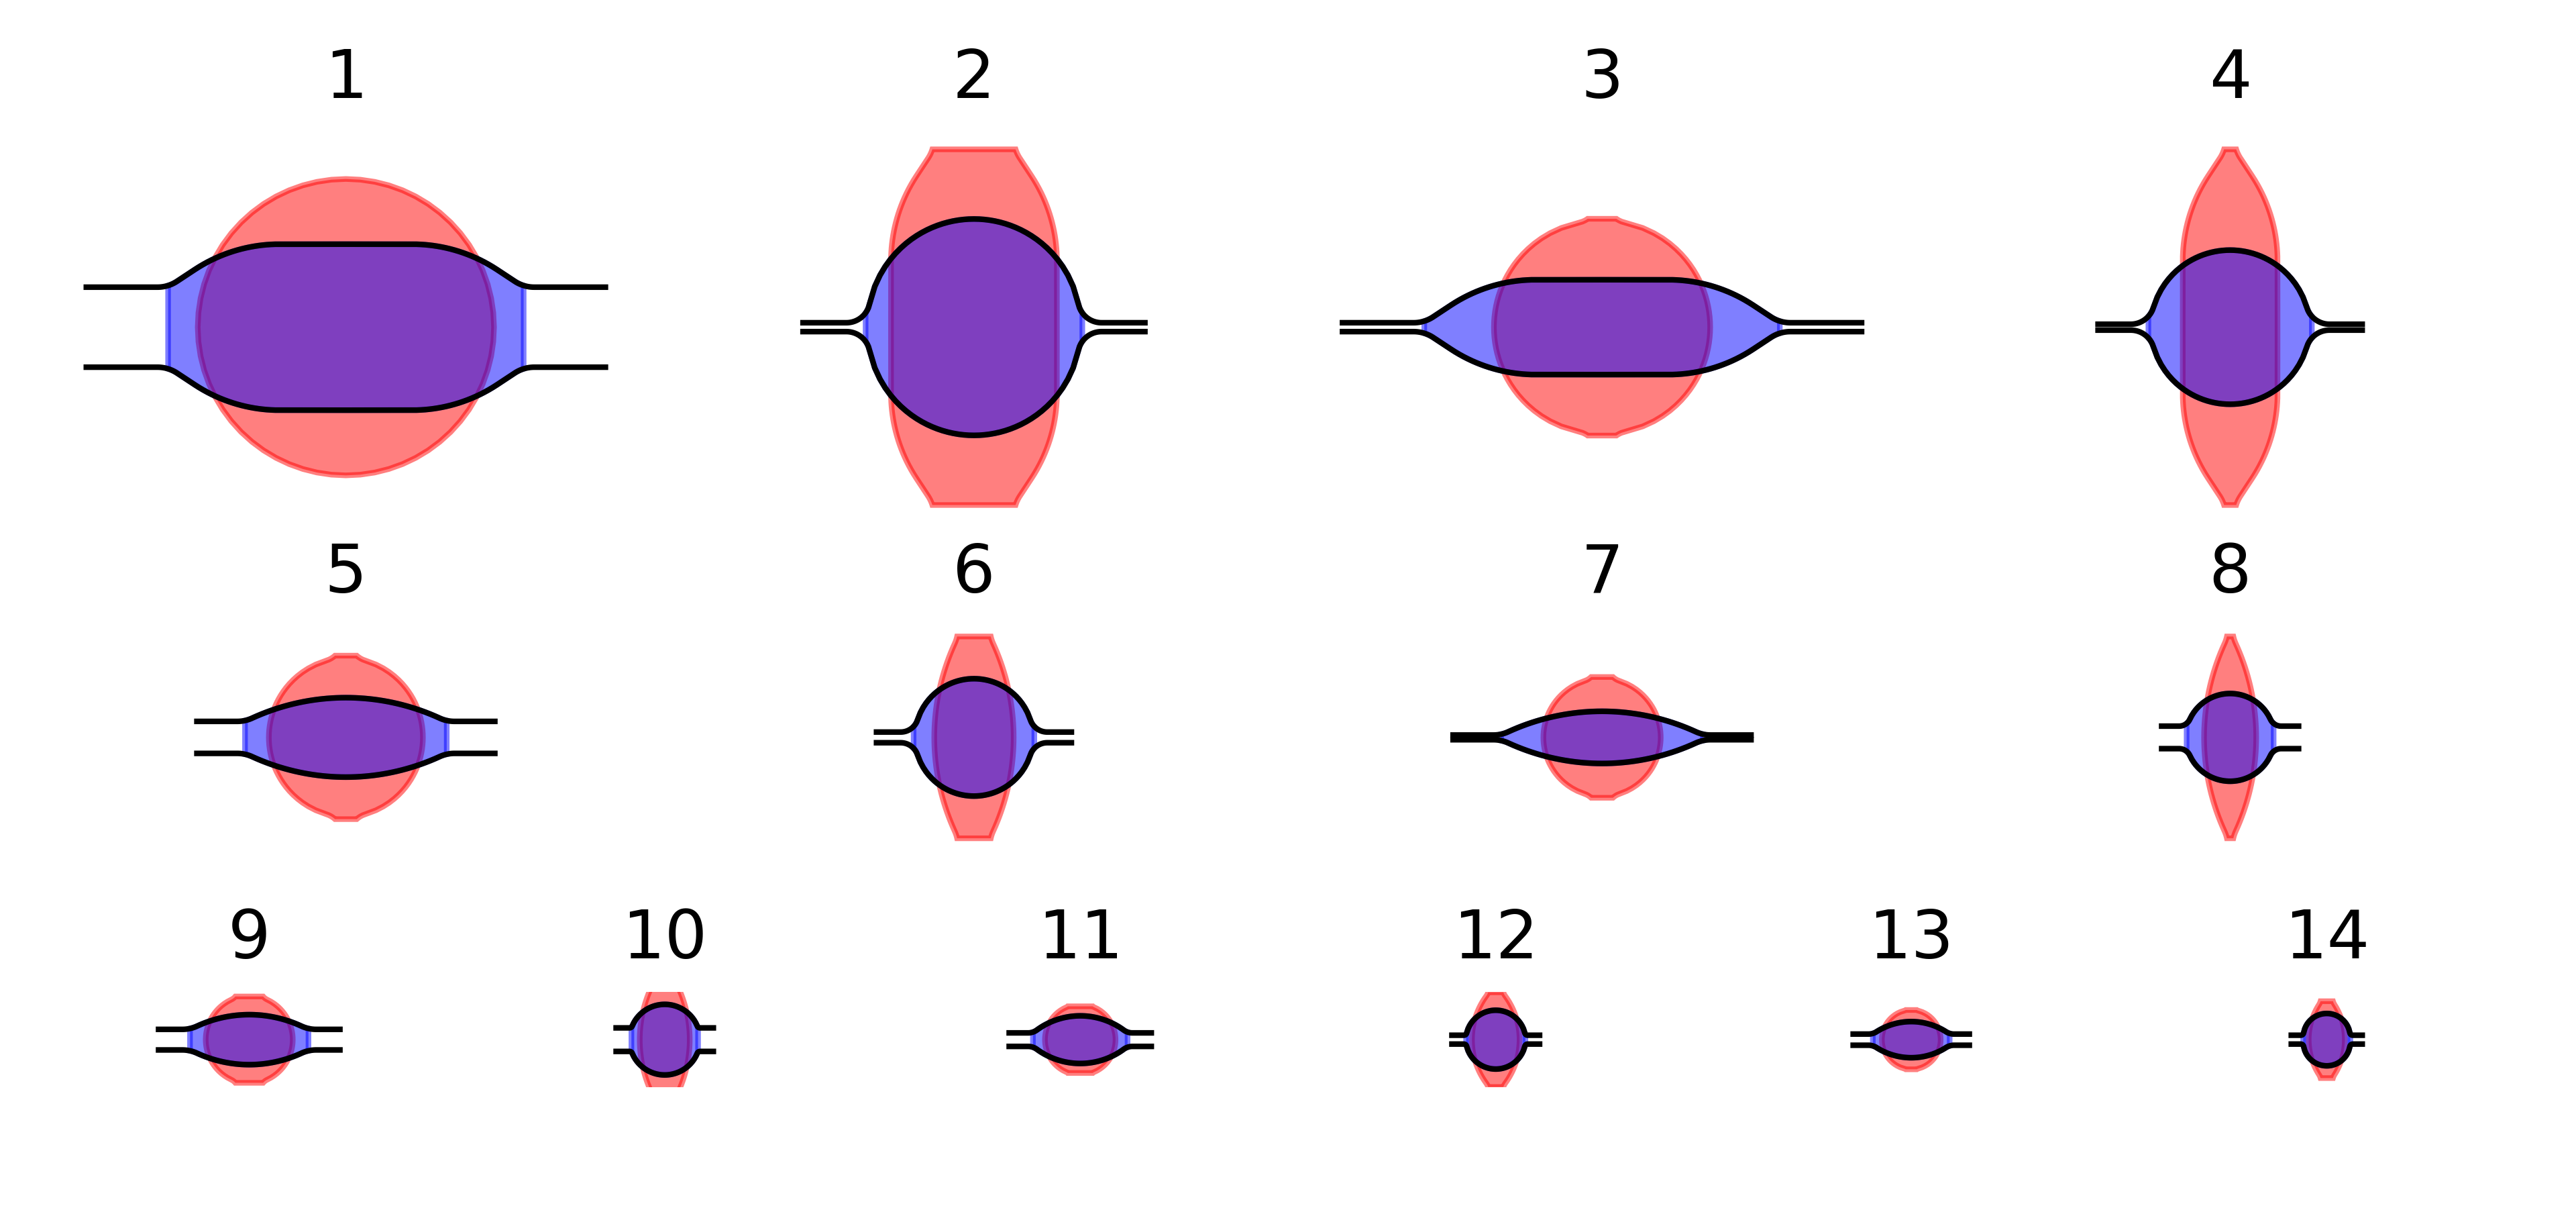
\includegraphics{img/plot_pass_sequence}
    \caption{True Scaled Illustration of the Investigated Pass Sequence}
    \label{fig:plot_pass_sequence}
\end{figure}


\begin{table}
    \centering
    \caption{Principal Data of the Investigated Pass Sequence}
    \label{tab:process_conditions}
    \begin{tblr}{colspec={l|XXXXXX}}
    \toprule
    \#             & Type                       & $\Width$                                               & $\Height$                                              & $\RollGap$                              & $\RollRadius$                                           & $\Velocity$                          \\
    &                            & \unit{\milli\meter}                                    & \unit{\milli\meter}                                    & \unit{\milli\meter}                     & \unit{\milli\meter}     & \unit{\meter\per\second}   \\
    \midrule
    
    {{ p.label }} & {{ p | format_pass_type }} & \num{ {{- (p.out_profile.width * 1e3) | round(1) -}} } & \num{ {{-  (p.out_profile.height * 1e3) | round(1) -}} } & \num{ {{-  (p.gap * 1e3) | round(1) -}} } & \num{ {{-  (p.roll.nominal_radius * 1e3) | round(1) -}} } & \num{ {{-  p.velocity | round(1) -}} }\\
    
    \bottomrule
\end{tblr}
\end{table}

Online measurements of the process conditions and workpiece state are done regarding roll force and torque, as well as workpiece temperature.
The latter is measured using pyrometers at several points in the plant: at entry and exit of the reversing stand and before, between and after the finishing stands.
The sensor signals are collected as timelines, so that they can be automatically analysed afterwards as described in \autoref{subsec:data-acquisition}.

To achieve statistical certainty, a number of 45 rolling trials were carried out.
This enables an estimation of the variations appearing.
A major source of variation in these trials is the manual feeding of the workpiece into the reversing passes.
The duration of those is scheduled with about 6 seconds.
The actual time needed has to be investigated in this work, see \autoref{subsec:data-acquisition} for details.

\subsection{Monte-Carlo Approach}\label{subsec:monte-carlo-approach}

\begin{figure}
    \centering
    \includegraphics[width=\linewidth]{img/chart_mc_principle}
    \caption{Chart of the Concept of Variation Estimation Using Monte Carlo Techniques}
    \label{fig:chart_mc_principle}
\end{figure}

The basic idea of the approach shown here is to simulate the rolling process several times with different input values, which are drawn by a random number generator according to predefined statistical distributions.
Afterwards, the distribution of the results can be analysed by classic methods of descriptive statistics to obtain information about the process' variational behavior.
The principle is shown in \autoref{fig:chart_mc_principle}.

This approach provides information about the overall variational behavior of the process.
If a single source of variation is introduced in the input, the reaction of the process on this variable can be analysed.
The count of variation sources introduced is generally unbounded.
In contrast to classic Taylor series error propagation, the computational effort does not directly increase remarkably with increasing count of investigated parameters.
However, an increase in sample size can be necessary to achieve sufficient certainty.
The key problem is to obtain data describing the variations of the input variables.
The tracing back of result variations to the input can be done using classic correlation methods of descriptive statistics, however, with the same typical caveats.
The main benefit of the approach is, that no information about the internals of the simulation procedure is needed for variational analysis, especially there is no need for derivatives of result values in dependence on the input.
The simulation procedure can generally be treated as black box with defined input and output interfaces.

\subsection{Statistical Data Acquisition}\label{subsec:data-acquisition}

As input for the Monte-Carlo approach statistical descriptions of the regarded input variables are needed.
Regarding the geometric variations of the input workpiece, the diameter of the samples was determined at multiple spots using a calibre.
The initial temperature of the samples was determined using the pyrometer installed near the roll gap entry.
Both were approximated using a normal distribution for sampling of random input values.

The question of varying inter-pass durations is crucial for scientific experiments on microstructure evolution, but currently often neglected.
Mostly, only fixed durations between the reversing passes are included in the design calculations.
Due to manual transport and feed of the workpiece to the following roll pass, the scheduled inter-pass durations are never realized in practice.
Although, these deviations from the schedule influence the microstructure evolution of the sample, as well as the actual conditions in the roll passes.
The current approach is aimed to help quantifying these deviations.

To obtain the inter-pass durations from the timeline data, the passes have to be identified automatically.
This was done by analysing the roll torque signal as plotted in \autoref{fig:plot_timeline_pass_finding}.
The original signal was first downsampled and smoothed.
Then, a difference filter was applied and the peaks of the resulting signal were determined.
These peaks denote start and end times of the roll passes, the middle time of those was used as time coordinate of the roll pass.
The distances of those were used as the inter-pass durations.

\begin{figure}
    \centering
    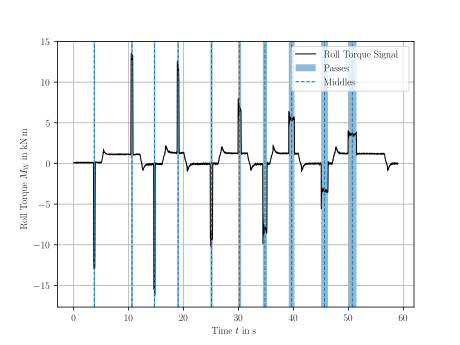
\includegraphics{img/plot_timeline_pass_finding}
    \caption{Example Roll Torque Signal With Automatically Determined Roll Pass Locations}
    \label{fig:plot_timeline_pass_finding}
\end{figure}

For the approximative description of the durations' distribution, a gamma distribution was used, which is a generalized exponential distribution.
The probability density function (PDF) of the gamma distribution is defined as in \autoref{eq:gamma-dist}, where $\Gamma$ is the gamma function and $\GammaDistributionAlpha > 0$ and $\GammaDistributionBeta > 0$ are parameters.

\begin{equation}
    f(x) = \frac{\GammaDistributionBeta^\GammaDistributionAlpha}{\Gamma(\GammaDistributionAlpha)}x^{\GammaDistributionAlpha - 1} \exp(-\GammaDistributionBeta x)
    \label{eq:gamma-dist}
\end{equation}

Since the gamma distribution is only defined for $x>0$, but no inter-pass durations below a certain value occur due to technical restrictions, the distribution was modified by introducing a minimal inter-pass duration $\Min{\Pause\Duration}$ with $x = \Pause\Duration - \Min{\Pause\Duration}$.
So there are three free parameters $\GammaDistributionAlpha$, $\GammaDistributionBeta$ and $\Min{\Pause\Duration}$ for fitting of the distribution function.
The fitting was done using least squares optimization of the PDF function on the density histogram of the data.

\subsection{Core Simulation Procedure}\label{subsec:simulation-procedure}

In the current work, the open-source rolling simulation framework PyRolL~\cite{pyroll2} was used to simulate the rolling process.
Generally, the shown approach can be used with every rolling simulation software available, since the procedure does not depend on any internals of the simulation.
A fast simulation approach, however, is favourable, since the simulation has to be done several, up to hundreds of, times.
The models used here are of one-dimensional type, thus, they lack of resolution in other directions as the rolling direction and provide only limited accuracy, but at the benefit of high solution speed.
They typically combine empirical approaches with simplified analytical solutions.
The simulation was done with the basic configuration of PyRolL, which includes the empirical roll force and torque model of \textcite{Hensel1978}, an integral thermal model approach according to \textcite{Hensel1990}, contact area estimation according to \textcite{Zouhar1960} and roll flattening according to \textcite{Hitchcock1935}.
Spreading was simulated using the equivalent flat pass according to \citeauthor*{Lendl1948}~\cite{Lendl1948, Lendl1948a, Lendl1949} in conjunction with the spreading equation of \textcite{Wusatowski1969}.
Details of software construction and model equations are provided in the documentation of PyRolL~\cite{pyroll}.


% TODO: kurze Beschreibung der wichtigsten Modelle: Thermik, Mikrostruktur, Hensel

The models most important for the following elaborations will be discussed in brief.
The temperature change of the workpiece was calculated by an integral heat balance as proposed by \textcite{Hensel1990} and given in \autoref{eq:heat-balance}.
%TODO: correct surface, capacity
\begin{equation}
    \Delta\Temperature = \Delta\Temperature_\Convection + \Delta\Temperature_\Contact + \Delta\Temperature_\Deformation + \Delta\Temperature_\Radiation
    \label{eq:heat-balance}
\end{equation}

\noindent$\Delta\Temperature_\Convection$ is the temperature change by convective heat flows according to \autoref{eq:heat-convection} with $\HeatTransferFactor_{\Convection}$ as a heat transfer factor, $\Temperature_\Environment$ as the environment temperature, $\Temperature$ as the current workpiece temperature and $\Duration$ as the duration of the process step.

\begin{equation}
    \Delta\Temperature_\Convection = \HeatTransferFactor_{\Convection} \left( \Temperature_\Environment - \Temperature \right) \Duration
    \label{eq:heat-convection}
\end{equation}

\noindent$\Delta\Temperature_\Contact$ is the temperature change by contact to the rolls according to \autoref{eq:heat-contact} with $\HeatTransferFactor_{\Contact}$ as a heat transfer factor and $\Temperature_{\Roll}$ as the temperature of the rolls.

\begin{equation}
    \Delta\Temperature_\Contact = \HeatTransferFactor_{\Contact} \left( \Temperature_\Roll - \Temperature \right) \Duration
    \label{eq:heat-contact}
\end{equation}

\noindent$\Delta\Temperature_\Radiation$ is the temperature change by radiation according to \autoref{eq:heat-radiation} with $\StefanBoltzmannCoefficient$ as the Stefan's and Boltzmann's constant and $\RelativeRadiationCoefficient$ as the relative radiation coefficient of the gray radiator.

\begin{equation}
    \Delta\Temperature_\Radiation = \StefanBoltzmannCoefficient \RelativeRadiationCoefficient \left( \Temperature_\Environment^4 - \Temperature^4 \right) \Duration
    \label{eq:heat-radiation}
\end{equation}

\noindent$\Delta\Temperature_\Deformation$ is the temperature change by deformation according to \autoref{eq:heat-deformation} with $\DeformationResistance$ as the empirical deformation resistance and $\Equivalent\LogStrain$ as the equivalent plastic strain.
Since the deformation resistance is used here instead of the flow stress, this term also includes approximately the heat generation by inner and outer friction.

\begin{equation}
    \Delta\Temperature_\Deformation = \num{0.95} \DeformationResistance \Equivalent\LogStrain
    \label{eq:heat-deformation}
\end{equation}

The deformation resistance was taken as proposed by \textcite{Hensel1978} and given in \autoref{eq:deformation-resistance}.

\begin{multline}
    \frac{\DeformationResistance}{\Equivalent\FlowStress} = \num{0.9901} + \num{0.106} \frac{\ContactArea}{\Equivalent\CrossSection} + \num{0.0283} \left( \frac{\ContactArea}{\Equivalent\CrossSection} \right)^2 + \num{1.5718} \exp \left[ \num{-2.4609} \frac{\ContactArea}{\Equivalent\CrossSection} \right] \\
    + \num{0.3117} \exp \left[ \num{-15.625} \left( \frac{\ContactArea}{\Equivalent\CrossSection} \right)^2 \right]
    \label{eq:deformation-resistance}
\end{multline}

The material data and model coefficients used above were taken for the following simulations as in \autoref{tab:material_data}.

\begin{table}
    \centering
    \caption{Material Data and Model COefficients Used in the Simulations}
    \label{tab:material_data}
    \begin{subtable}{\linewidth}
    \caption{Flow Stress Model of C45 acc.~to~\cite{Spittel2009}}
    \begin{tblr}{
        colspec={XXXXX},
        columns={r},
        row{1}={1cm,m},
        row{2}={l},
        row{4}={l},
        cell{1}{1} = {c=7}{c},
        cell{4-5}{4,6} = {c=2}{},
    }
        \toprule
        $\displaystyle \FlowStress = \FlowStressA \cdot \E^{\FlowStressM1 \CelsiusTemperature} \cdot \LogStrain^{\FlowStressM2} \cdot \LogStrainRate^{\FlowStressM3} \cdot \E^{\FlowStressM4/\LogStrain} \cdot \left( 1 + \LogStrain \right)^{\FlowStressM5\CelsiusTemperature + \FlowStressM6} \cdot \E^{\FlowStressM7\LogStrain} \cdot \left( 1 + \LogStrainRate \right)^{\FlowStressM8\CelsiusTemperature} \cdot \CelsiusTemperature^{\FlowStressM9}$ \\
        $\FlowStressA$ & $\FlowStressM{{- i -}}$ \\
            \midrule
            \num{ {{- c.a / 1e6 -}} } & \num{ {{- c["m{}".format(i)] -}} } \\[3mm]
            $\FlowStressM{{- i -}}$ &  $\CelsiusTemperature$ && $\LogStrain$ \\
            \midrule
            \num{ {{- c["m{}".format(i)] -}} } &  \qtyrange{820}{1200}{\celsius} && \numrange{0.04}{1.5}\\
            \bottomrule
    \end{tblr}
\end{subtable}
\\\vspace{1em}
\begin{subtable}{\linewidth}
    \caption{Parameters for Generalized JMAK Model as in Equations~\ref{eq:jmak-fraction} to~\ref{eq:jmak-grain-size} acc.~to \textcite{Hodgson1992}}
    \begin{tblr}{
        colspec={llXXXX},
        columns={r},
        row{1}={l},
        column{1-2}={l},
    }
        \toprule
        Mechanism & Parameter & 1 & 2 & 3 & 4 \\
        \midrule
        Dynamic
        & $a$ & \num{ {{- "{:.2e}".format(drx.a1) -}} } & \num{ {{- drx.a2 -}} } & \num{ {{- drx.a3 -}} } & \num{ {{- drx.a4 -}} } \\
        & $b$ & \num{ {{- "{:.2e}".format(drx.b1) -}} } & \num{ {{- drx.b2 -}} } & \num{ {{- drx.b3 -}} } & \num{ {{- drx.b4 -}} } \\
        & $c$ & \num{ {{- "{:.2e}".format(drx.c1) -}} } & \num{ {{- drx.c2 -}} } & \num{ {{- drx.c3 -}} } & \num{ {{- drx.c4 -}} } \\
        Meta-Dynamic
        & $a$ & \num{ {{- "{:.2e}".format(mrx.a1) -}} } & \num{ {{- mrx.a2 -}} } & \num{ {{- mrx.a3 -}} } & \num{ {{- mrx.a4 -}} } \\
        & $b$ & \num{ {{- "{:.2e}".format(mrx.b1) -}} } & \num{ {{- mrx.b2 -}} } & \num{ {{- mrx.b3 -}} } & \num{ {{- mrx.b4 -}} } \\
        & $c$ & \num{ {{- "{:.2e}".format(mrx.c1) -}} } & \num{ {{- mrx.c2 -}} } & \num{ {{- mrx.c3 -}} } & \num{ {{- mrx.c4 -}} } \\
        Static
        & $a$ & \num{ {{- "{:.2e}".format(srx.a1) -}} } & \num{ {{- srx.a2 -}} } & \num{ {{- srx.a3 -}} } & \num{ {{- srx.a4 -}} } \\
        & $b$ & \num{ {{- "{:.2e}".format(srx.b1) -}} } & \num{ {{- srx.b2 -}} } & \num{ {{- srx.b3 -}} } & \num{ {{- srx.b4 -}} } \\
        & $c$ & \num{ {{- "{:.2e}".format(srx.c1) -}} } & \num{ {{- srx.c2 -}} } & \num{ {{- srx.c3 -}} } & \num{ {{- srx.c4 -}} } \\
        \bottomrule
    \end{tblr}
\end{subtable}
\\\vspace{1em}
\begin{subtable}{\linewidth}
    \caption{Other Material Data and Model Coefficients}
    \begin{tblr}{
        colspec={XXXXX},
        columns={r},
        row{1-2}={l},
    }
        \toprule
        $\Density$                                  & $\ThermalCapacity$                                   & $\Contact{\HeatTransferFactor}$                        & $\Convection{\HeatTransferFactor}$ & $\RelativeRadiationCoefficient$                    \\
        \unit{\kilo\gram\per\cubic\meter}           & \unit{\joule\per\kilo\gram\per\kelvin}               & \unit{\watt\per\square\meter\per\kelvin} & \unit{\watt\per\square\meter\per\kelvin} & \\
        \midrule
        \num{ {{- "{:.1f}".format(ip.density) -}} } &
        \num{ {{- "{:.1f}".format(ip.specific_heat_capacity) -}} } &
        \num{ {{- "{:.1f}".format(alpha_cont) -}} } &
        \num{ {{- "{:.1f}".format(alpha_conv) -}} }  &
        \num{ {{- "{:.1f}".format(epsr) -}} } \\
        \bottomrule
    \end{tblr}
\end{subtable}

\end{table}

